\begin{center}
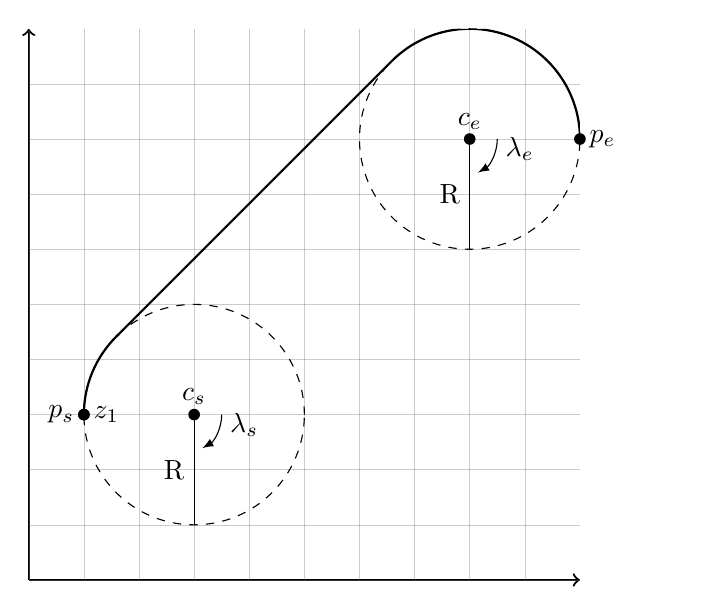
\begin{tikzpicture}
	[scale=7,
	axis/.style={->,black,thick}]
	
	% Draw main axes
	\draw[axis] (0,0) -- (1,0);
	\draw[axis] (0,0) -- (0,1);

	% Draw grid
	\foreach \x in {0,0.1,...,1}
		\foreach \y in {0,0.1,...,1}
		{
			\draw[very thin, gray, opacity=0.05] (\x, 0) -- (\x, 1);
			\draw[very thin, gray, opacity=0.05] (0, \y) -- (1, \y);
		}

	% Create circles
	\coordinate (C1) at (0.3, 0.3);
	\coordinate (C2) at (0.8, 0.8);
		
	\fill (C1) circle[radius=0.3pt] node[anchor=south]{$c_s$};
	\fill (C2) circle[radius=0.3pt] node[anchor=south]{$c_e$};

	\draw[dashed] (C1) circle(0.2);
	\draw[dashed] (C2) circle(0.2);
	
	% Create waypoints
	\coordinate (START) at (0.1, 0.3);
	\coordinate (END) at (1, 0.8);
	
	\fill (START) circle[radius=0.3pt] node[anchor=east]{$p_s$};
	\fill (END) circle[radius=0.3pt] node[anchor=west]{$p_e$};

	% Draw path
	\coordinate (Z1) at (0.15858, 0.44142);
	\begin{scope}
		\path[clip] (C1) -- (0.16, 0.45) -- (0.0, 0.3);
		\draw[thick] (C1) circle (2mm);
	\end{scope}
	
	\coordinate (Z2) at (0.65858, 0.94142);
	\begin{scope}
		\path[clip] (C2) -- (0.6, 1.0) -- (1.2, 1.0);
		\draw[thick] (C2) circle (2mm);
	\end{scope}
	
	\begin{scope}
		\path[clip] (C2) -- (1.0, 0.9) -- (1.0, 0.8);
		\draw[thick] (C2) circle (2mm);
	\end{scope}
	
	\draw[thick] (Z1) -- (Z2);

	
	% Create radiusesesesess
	\draw (0.3, 0.3) -- (0.3, 0.1) node[midway, anchor=east]{R};
	\draw (0.8, 0.8) -- (0.8, 0.6) node[midway, anchor=east]{R};

	% Draw direction
	\draw[-latex] (0.35,0.3) arc (0:-60:2.0pt) node[near start,right] {$\lambda_s$};
	\draw[-latex] (0.85,0.8) arc (0:-60:2.0pt) node[near start,right] {$\lambda_e$};
	
	% First half plane
	\fill (START) circle[radius=0.3pt] node[anchor=west]{$z_1$};
	
	

\end{tikzpicture}
\end{center}